\documentclass[fontsize=11pt]{scrartcl}
%-------------------------------------------------------------------------------------------------
% LATEX TEMPLATE FOR A BACHELOR'S THESIS AT GHENT UNIVERSITY GLOBAL CAMPUS
% CREATED BY MANVEL GASPARYAN
% APRIL, 2021
%-------------------------------------------------------------------------------------------------
\usepackage{hyperref, tikz, float, subfigure, multicol, amsmath, amsthm, alphalph, amsfonts, amssymb, geometry, enumitem, parskip, xcolor, sectsty}
\usepackage[normalem]{ulem}
\usepackage[font=scriptsize,labelfont=bf]{caption}
\usepackage[explicit]{titlesec}
\usepackage[scaled]{helvet}
\renewcommand\familydefault{\sfdefault} 
\usepackage[T1]{fontenc}

\usepackage{setspace}

\usepackage{{listings}}

%-------------------------------------------------------------------------------------------------
 \geometry{a4paper, total={170mm,257mm}, left=20mm, right=20mm, top=25mm, bottom=30mm}
%-------------------------------------------------------------------------------------------------
\newtheorem{proposition}{Proposition}[section]
\newtheorem{lemma}{Lemma}[section]
\newtheorem{remark}{Remark}[section]
\newtheorem{corollary}{Corollary}[section]
\newtheorem{definition}{Definition}[section]
%-------------------------------------------------------------------------------------------------
\pagenumbering{roman}
\usepackage{fancyhdr}
\pagestyle{fancy}
\fancyhf{}
\renewcommand{\headrulewidth}{0pt}
\rhead{}
\lhead{}
\rfoot{\thepage}
\lfoot{}

%-------------------------------------------------------------------------------------------------
\definecolor{ghent_blue}{rgb}{0.1176, 0.392, 0.7843}
\definecolor{ghent_dark}{rgb}{0.0, 0.2, 0.4}
%-------------------------------------------------------------------------------------------------
\title{{\color{ghent_blue} TITLE: LATEX TEMPLATE FOR A BACHELOR'S THESIS AT GHENT UNIVERSITY GLOBAL CAMPUS}}
\subtitle{{\color{ghent_dark} [DOCUMENT SUBTITLE]}}
\date{}         
%-------------------------------------------------------------------------------------------------
\sectionfont{\fontsize{16}{15}\selectfont}
\sectionfont{\color{ghent_blue}}
%=================================================================================================
\begin{document}
%=================================================================================================
%PAGE i: TITLE PAGE 1
%-------------------------------------------------------------------------------------------------
\thispagestyle{empty}
\hfill
\includegraphics[scale = 1]{img/badge/2021.png}\\
%-------------------------------------------------------------------------------------------------
\vspace{8cm}

\noindent{\fontsize{30}{50}\selectfont{\color{ghent_blue}\noindent \hspace{12mm}\textbf{
Microphotonics %TITLE
}}}\\
\fontsize{20}{50}\selectfont{\color{ghent_dark}\noindent \hspace{13mm}\textbf{
CAD-LAB: TASK NAME%SUBTITLE
}}\vspace{10mm}

\hspace{10mm}{\fontsize{10}{10}\selectfont{\textbf{
Farima Mehrzan, Lukuan Zhang, Rui Zhu, Xiyuan Guo%AUTHOR
}}}
\vspace*{\fill}
%-------------------------------------------------------------------------------------------------
\begin{flushleft}
\begin{figure}[b!]

\includegraphics[scale = 1.4]{img/badge/GUGC.pdf}
\end{figure}
\end{flushleft}

\doublespacing
\tableofcontents
\pagebreak
\pagenumbering{arabic}
%=================================================================================================
%HELP
%-------------------------------------------------------------------------------------------------
\section*{*  \uline{HELP}}
Once have been refered you can delete this part.\\
If you want to write an inline equation, code like this $E=mc^2$.\\
If you want to write a displayed equation without numbering, code like this $$E=mc^2$$\\
If you want to write a numbering displayed equation, code like this
\begin{equation} 
    E=mc^2 \label{eq1}
\end{equation}
and you can quote the equation by using Eq.\ref {eq1}.\\
\textbf{Tips:} The software \verb|Mathpix| can convert images and PDFs to LaTeX format which is
highly recommended by me.\\
List items like this:
\begin{enumerate} % itemize/description
    \item contents
    \item contents
\end{enumerate}
If you want to add one or more images as Figure \ref{name1} shown, you can copy the
code as following.\\
\begin{figure}[H]
    \centering
     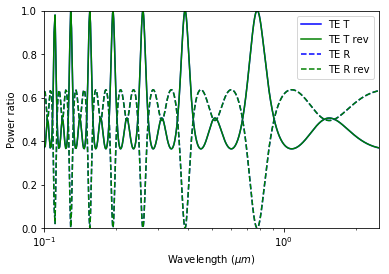
\includegraphics[width=0.35\textwidth]{img/1.png} % set width to get a proper ratio
     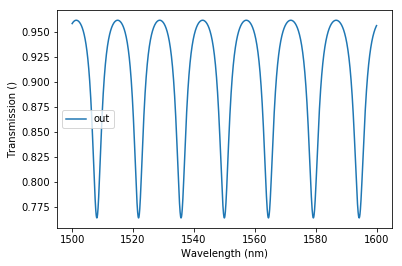
\includegraphics[width=0.35\textwidth]{img/2.png}
     \caption{Here to write the caption of the figure.}
     \label{name1}
\end{figure}
{\color{ghent_blue}Some details to notice:}
\begin{enumerate}
    \item  \textbf{Function name} and \textbf{units} should be presented in the Roman Regular Font.
    We can do this by using the sign backslash such as $\log(x)$, $\sin(x)$, $\cos(x)$, etc.
    \item When writing source codes in \LaTeX, make sure that the one-line code length 
    \textbf{does not} exceed one page(or 1/2 screen width on computer). Too long in width makes 
    a worse reading experience.
    \item Everytime when the new task comes, you are allowed to copy the whole template file and 
    rename it into the task name, then modify on the copy. Please don't modify the code directly
    on the template.
    \item Don't forget enter a space after the punstuation marks.
\end{enumerate}



%=================================================================================================
\pagebreak
%=================================================================================================
\section{Task 1}
\subsection{Design of the filter}
The ring length of the single-ring single-waveguide filter that has a resonance at
1.55$\mu m$, and six other ones - between 1.5 $\mu m$ and 1.6 $\mu m$ is given by,\\
\begin{equation}
    2L=\frac{m\lambda}{n_{eff}}, 96\leq m\leq 120
    \label{2L_1}
\end{equation}
There are total 25 ring lengths that meet the requirement from 55.111$\mu m$ to 68.889$\mu m$. \\
\textbf{Method to calculation}\\
The filter has a resonance at $\lambda=1.55\mu m $,so we have,\\
\begin{equation}
    \lambda=\frac{2Ln_{eff}} m , m\in N_+  
\end{equation}
where $\lambda=1.55\mu m,n_{eff}=2.7$.
The third and fourth wavelength before or after $1.55\mu m$ when the filter has a resonance is,
\begin{equation}
    \begin{array}[]{lr}
    \lambda_1=\frac{2Ln_{eff}}{m+3},\lambda_1'=\frac{2Ln_{eff}}{m+4} \\
    \lambda_2=\frac{2Ln_{eff}}{m-3},\lambda_2'=\frac{2Ln_{eff}}{m-4}
    \end{array}
\end{equation}
We need to make sure that there are exactly seven wavelengths of resonance point between 1.5 $\mu m$ and 1.6 $\mu m$,
\begin{equation}
    \left\{ 
        \begin{array}[]{lr}
             \lambda_1 \geq 1.5 \mu m, \lambda_1'<1.5\mu m\\
             \lambda_2 \leq 1.6 \mu m, \lambda_2'>1.6\mu m 
        \end{array}
   \right.
\end{equation}
After calculation, we get $96\leq m\leq 120$ and $55.111\mu m\leq 2L\leq 68.889\mu m$ with $2L=\frac{m\lambda}{n_{eff}}$.
\begin{figure}[ht]
    \centering
    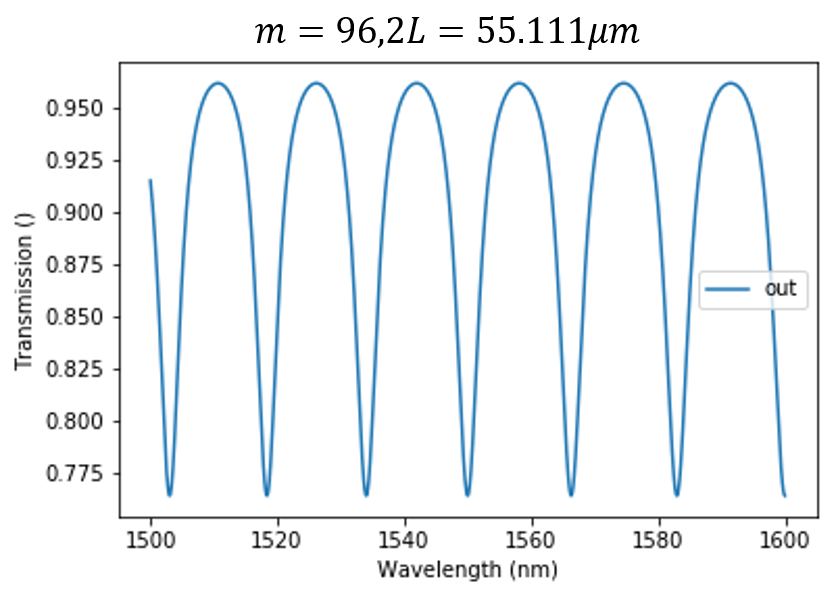
\includegraphics[width=0.3\textwidth]{img/t1_n96.png}
    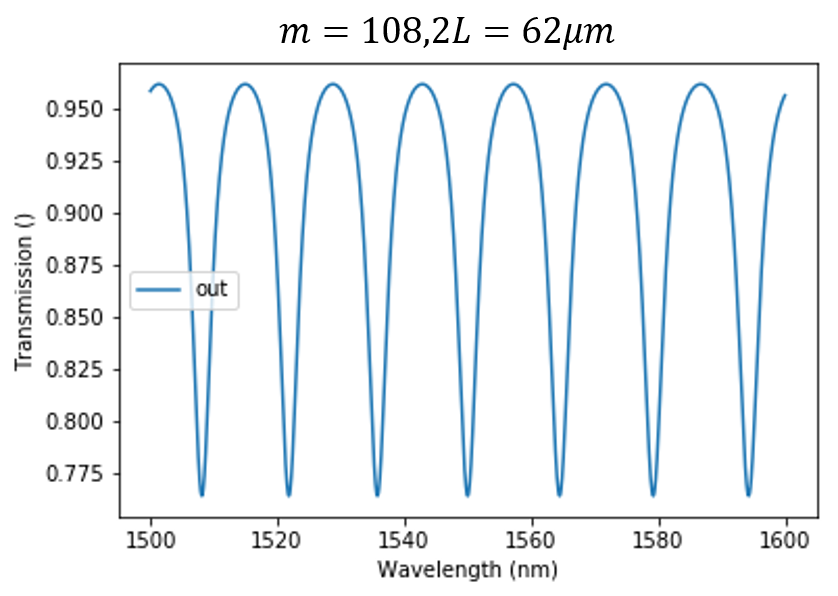
\includegraphics[width=0.3\textwidth]{img/t1_n108.png}
    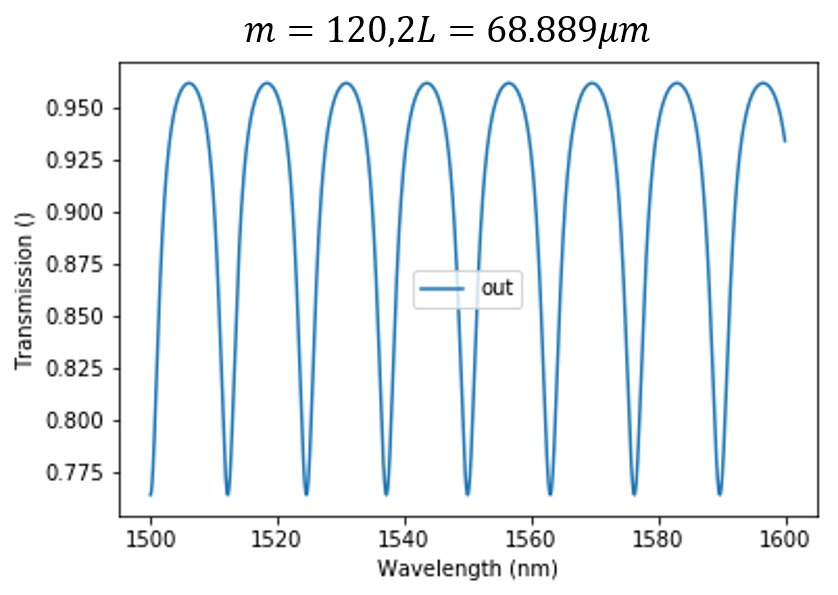
\includegraphics[width=0.3\textwidth]{img/t1_n120.png}
    \caption{Pass transmission with respect to wavelength}
    \label{t1_tp}
\end{figure}
The pass transmission is shown in Figure \ref{t1_tp}, when the ring length is equal to $55.111\mu m, 62\mu m,68.889\mu m$ ,respectly.
Obviously, each of them has seven resonances between 1.5 $\mu m$ and 1.6 $\mu m$ with one at 1.55$\mu m$.
So there is a resonance when $\lambda=\frac{2Ln_{eff}} m$. 2L is given by \ref{2L_1}.\\
From preparation, we know,
\begin{equation}
    \begin{split}
        T_p & =\frac{\tau^2+A^2-2A\tau \cos{\phi}}{1+A^2\tau^2-2A\tau\cos{\phi}}  \\
            & =1+\frac{\tau^2+A^2-1-A^2\tau^2}   {1+A^2\tau^2-2A\tau\cos{\phi}}
    \end{split}
\end{equation}
$\tau^2+A^2-1-A^2\tau^2=\kappa^2(A^2-1)<0$,so when $\cos \phi=1$,$T_p$,is minimum.\\
\textbf{Free spectral range}
\begin{equation}
    \Delta\lambda_{FSR}=\frac{\lambda^2}{2n_gL}
\end{equation}
In fact, the free spectral range(FSR) will change as the wavelength. If choosing $\lambda$ fixed, this format is not exact so much.
When we use the wavelength at the specific FSR to calculate $\Delta\lambda_{FSR}$, it is quite exact.\\
For example, as for the case of$2L=62\mu m$, it is shown in the center of Figure \ref{t1_tp}.$\Delta\lambda_{FSR}~=14.29 nm$.\\
\textbf{Critical coupling}   \\
Here, we choose $2l=62\mu m$. Obviously, only when $|\tau |=\exp{-2\alpha L}$, $T_p=0$ at wavelength of resonance,as shown in Figure \ref{t1_tp_critical}.
\begin{figure}[ht]
    \centering
    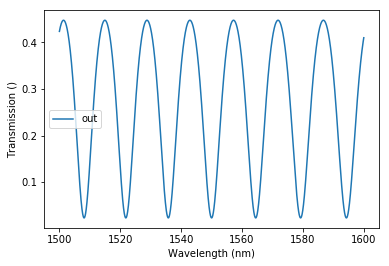
\includegraphics[width=0.3\textwidth]{img/T1_ccs.png}
    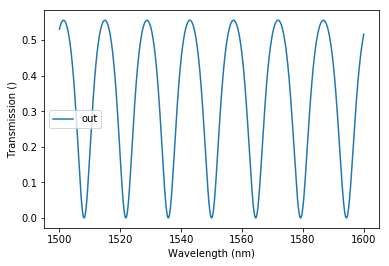
\includegraphics[width=0.3\textwidth]{img/T1_cc.png}
    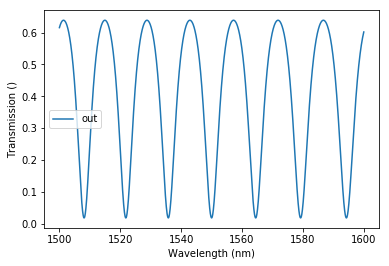
\includegraphics[width=0.3\textwidth]{img/T1_ccl.png}
    \caption{Pass transmission with respect to wavelength.When $\exp{-2\alpha:}<|\tau|$(left);When$\exp{-2\alpha:}=|\tau|$(center);When $\exp{-2\alpha:}>|\tau|$(right)}
    \label{t1_tp_critical}
\end{figure}


%%%%%%%%%%%%%%%%%%%%%%%%%%%%%%%%%%%%%%%%%%%%%%%%%%%%%%%%%%%%%%%%%%%%%%%%%%%%%%%%%%%%%%%%%%%%%%%%%%%%%%%%%%%%%%%%%%%%%%%%%%%%%%%%%%%%%%%%%%%%%%%%%%%%%%%%%
\section{Task 2}
\subsection{}
\begin{figure}[htbp]
    \centering
    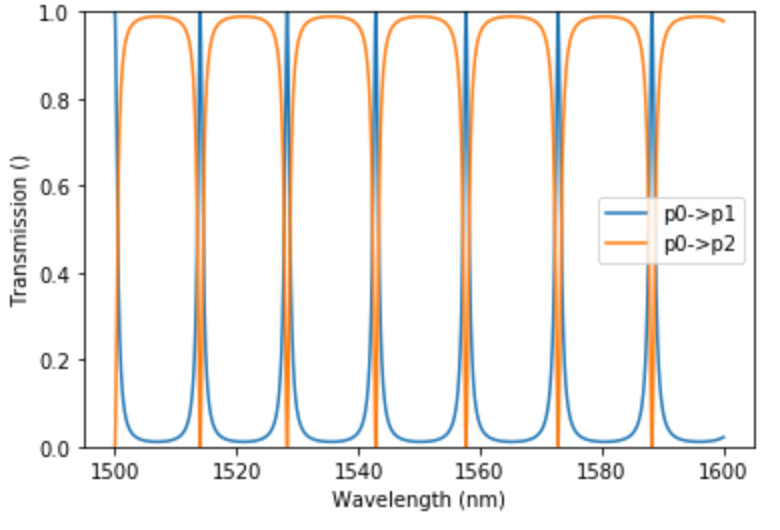
\includegraphics[width=0.5\textwidth]{img/T2_1.png}
    \caption{Transmission distribution of drop (blue) and pass (orange),ring length=60 $\mu m$}
    \label{t2_1}
\end{figure}
The figure \ref{t2_1} illustrates that maximum drop transmission and minimum pass transmission is at wavelengths ,
such as about 1500nm , 1514nm, 1528nm, 1542nm, 1558nm.
\subsection{}
\begin{figure}[h]
    \centering
    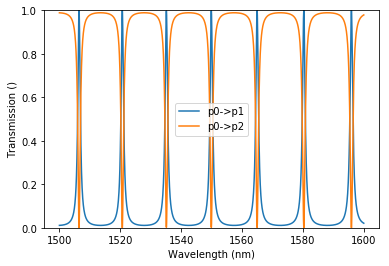
\includegraphics[width=0.5\textwidth]{img/T2_2.png}
    \caption{Transmission distribution of drop (blue) and pass (orange),ring length=59.7$\mu m$}
    \label{t2_2}
\end{figure}
As we solved in the preparation,the condition to obtain maximum 
$T_d $ is$ 2\beta L=2\pi m$ (m is positive integer).
Therefore,the ring length $2L=(mλ_0)/n_{eff} $. 
 For $λ_0  =1.55\mu m,n_{eff} =2.7$, l choose m=104,which makes 2L=59.7um .From figure \ref{t2_2},we can see resonance is around 1.55 $\mu m$.
 \subsection{}
 \begin{figure}[ht]
    \centering
    \subfigure[Bottom $\tau$=0.9 ,top $\tau$=0.9]{
    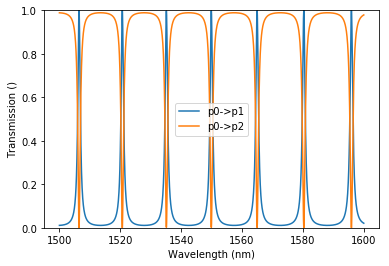
\includegraphics[width=5.5cm]{img/11.png}
    %\caption{fig1}
    }
    \quad
    \subfigure[Bottom $\tau$=0.9 ,top $\tau$=0.9]{
    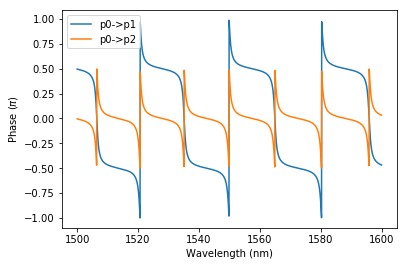
\includegraphics[width=5.5cm]{img/12.png}
    }
    \quad
    \subfigure[Bottom $\tau$=0.7 ,top $\tau$=0.9]{
    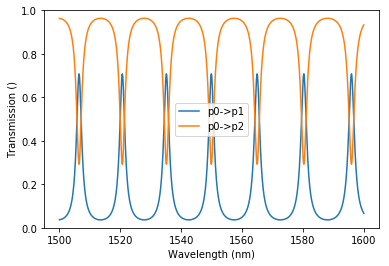
\includegraphics[width=5.5cm]{img/21.png}
    }
    \quad
    \subfigure[Bottom $\tau$=0.7 ,top $\tau$=0.9]{
    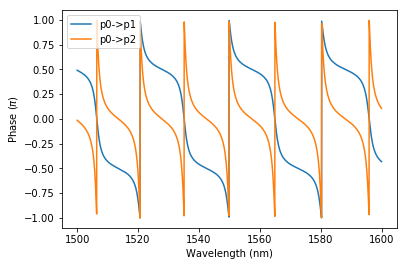
\includegraphics[width=5.5cm]{img/22.png}
    }
    \quad
    \subfigure[Bottom $\tau$=0.9 ,top $\tau$=0.7]{
    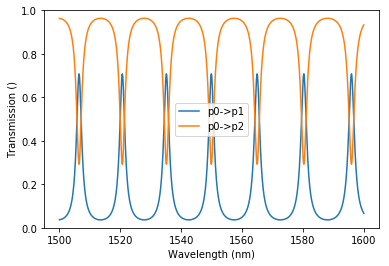
\includegraphics[width=5.5cm]{img/31.png}
    }
    \quad
    \subfigure[Bottom $\tau$=0.9 ,top $\tau$=0.7]{
    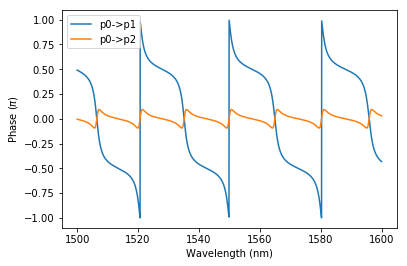
\includegraphics[width=5.5cm]{img/32.png}
    }

    \caption{Transmission(left) and phase(right) distribution of dfifferent 'unbalanced' rings}
    \label{T2b}
    \end{figure}
    From Figure \ref{T2b} (a) and (c), we can know the 'unbalanced' ring induces the maximum drop transmission decline sharply .
    Figure\ref{T2b} (b) and (c) illustrate the same contribution.
    Thus ,when we get an 'unbalanced' figure like (b) and (c) in practice, 
    we can't confirm which coupler have fabrication errors. 
    But it can be confirmed easily by check the phase distribution.
    When bottom $\tau$ = top $\tau$ , the phase of difference between the maximum and minimum is $\pi$ .
    When bottom $\tau$ < top tau or bottom $\tau$ $>$ top$ tau $, 
    the phase of difference between the maximum and minimum is respectively larger than $\pi$ orsmaller than $\pi$.
 \subsection{}
 \begin{figure}[h]
    \centering
    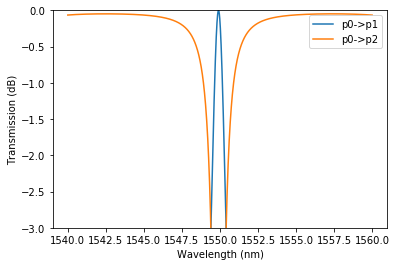
\includegraphics[width=0.5\textwidth]{img/T2_3.png}
    \caption{Transmission distribution (dB) of drop (blue) and pass (orange),ring \\
    length=59.7um,wavelength (1.54um, 1.56um)}
    \label{t2_2}
\end{figure}
For ring\_loss\_dB\_m=0,we can get A=0.The formula of $\Delta \lambda \_{3dB}$ can be simplified as:
\begin{equation}
    \Delta \lambda _{3dB}=\frac{(1-\tau^2)\lambda^2}{\tau \pi 2Ln_g}
\end{equation}
For no dispersion will be included so the effective index equals the group index,$n_{neff}=n_g=2.7$.
And  2L=59.7um,τ=0.9, λ =1.55um.Take parameters in the formula we get :
$$\Delta \lambda _{3dB}=1.00158 nm $$
From figure 2.4 ,we can see the bandwidth ,the distance between orange curve, 
is the same as the theoretical value of $\Delta \lambda _{3dB}$. 
\pagebreak
%=================================================================================================
%TASK 3
%-------------------------------------------------------------------------------------------------
\section{\uline{Multiple rings}}
%-------------------------------------------------------------------------------------------------
% Here comes some text. This text makes use of 1.5 line spacing. 
%-------------------------------------------------------------------------------------------------
%-------------------------------------------------------------------------------------------------
\subsection{}
%-------------------------------------------------------------------------------------------------
Set $m_1=110$ in $2\beta L = 2\pi m_1 \lambda$ in the first filter, 
$m_2$ in $2\beta L = 2\pi m_2 \lambda$
which respectively correspond to the ring length $2L_1 = 63.15\mathrm{\mu m}$
and $2L_2 = \frac{m_2}{m_1}\times 63.15\mathrm{\mu m}$. 
Assume there is no loss, the free spectral range and the 3dB-bandwidth
of the first ring
are given by:
\begin{equation}
    {\Delta \lambda_{F S R}}_1=\frac{\lambda^{2}}{2 n_{g} L_1}
\end{equation}
\begin{equation}
    \Delta \lambda_{3 d B}=\frac{\left(1-\tau^{2}\right) \lambda^{2}}{\tau  \pi 2 L_1 n_{g}}
\end{equation}
and in the same way we can get ${\Delta \lambda_{F S R}}_2$.
In order to filter the lights of which wavelengths are near $1550 \mathrm{nm}$,
consider the free spectral range of the second filter 
${\Delta \lambda_{F S R}}_2$ is 
at least smaller or longer of $3\Delta \lambda_{3 d B}$.
The relations are represented by:
\begin{equation}
    \begin{aligned}
    {\Delta \lambda_{F S R}}_2&>{\Delta \lambda_{F S R}}_1 + 3\Delta \lambda_{3 d B}, \mathrm{or}\\
    {\Delta \lambda_{F S R}}_2&<{\Delta \lambda_{F S R}}_1 - 3\Delta \lambda_{3 d B}
    \end{aligned}
\end{equation}
Then we get
\begin{equation}
    m_1 \le 91 \quad \mathrm{or} \quad m_1 \ge 138
\end{equation}
Figure \ref{fig3.1} shows the filtering results when $m_2=91, L_2=52.55 \mathrm{\mu m}$ 
or $m_2=138, L_2=79.09 \mathrm{\mu m}$.
Obviously resonances next to $\lambda=1.55\mathrm{\mu m}$ are effectively
removed.
\begin{figure}[H]
    \centering
    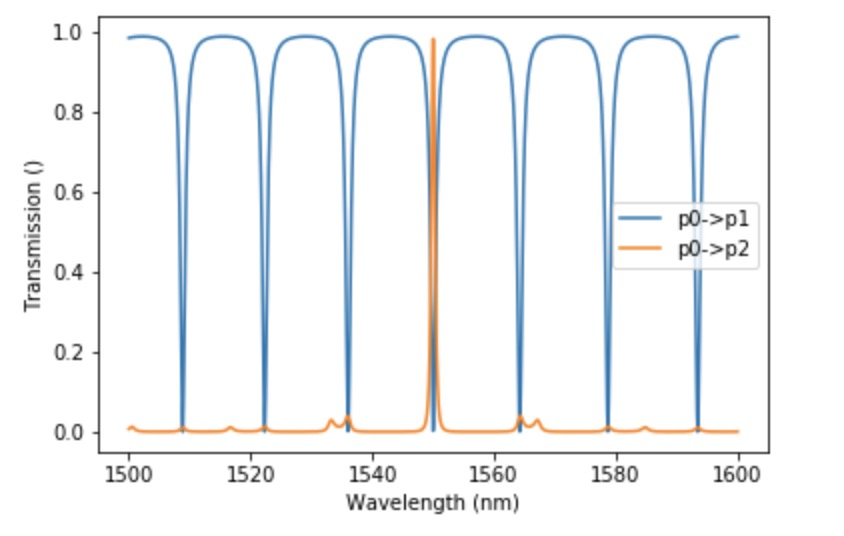
\includegraphics[width=0.4\textwidth]{img/fig3.1a.png}
    \hspace{0.5cm}
    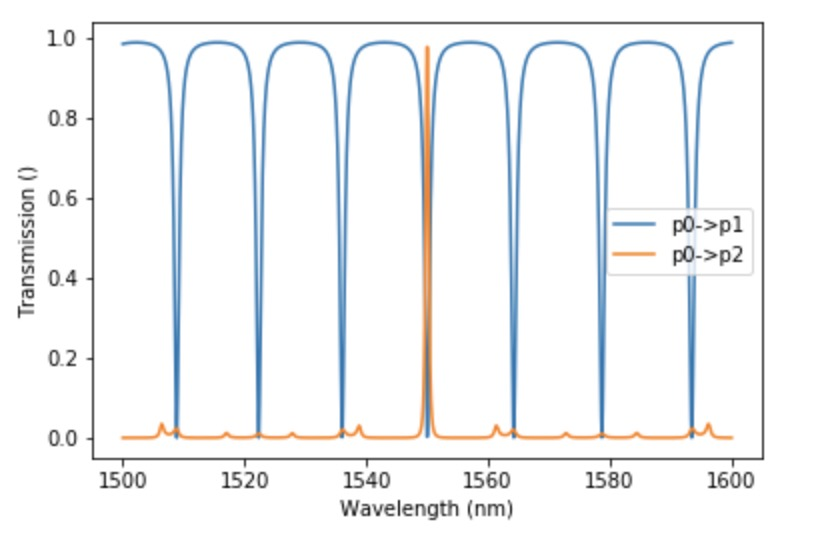
\includegraphics[width=0.4\textwidth]{img/fig3.1b.png}
    \caption{The transimission when $L_2=52.55 \mathrm{\mu m}$(left) 
    or $L_2=79.09 \mathrm{\mu m}$(right)}
    \label{fig3.1}
\end{figure}

\subsection{}
%-------------------------------------------------------------------------------------------------
When $\tau = \tau_{\mathrm{middle}}=0.9$, we observe the appearence of 
two peaks in Figure \ref{fig3.2}
\begin{figure}[H]
    \centering
    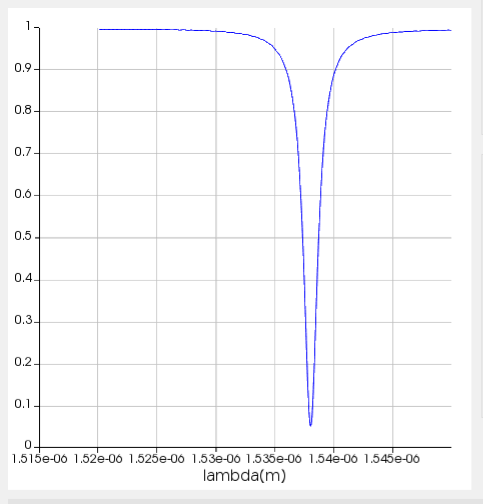
\includegraphics[width=0.4\textwidth]{img/fig3.2.png}
    \caption{The transimission when $\tau = \tau_{\mathrm{middle}}=0.9$}
    \label{fig3.2}
\end{figure}

By changing both $tau$ and $\tau_{\mathrm{middle}}$ we get Figure \ref{fig3.3}.

\begin{figure}[H]
    \centering
    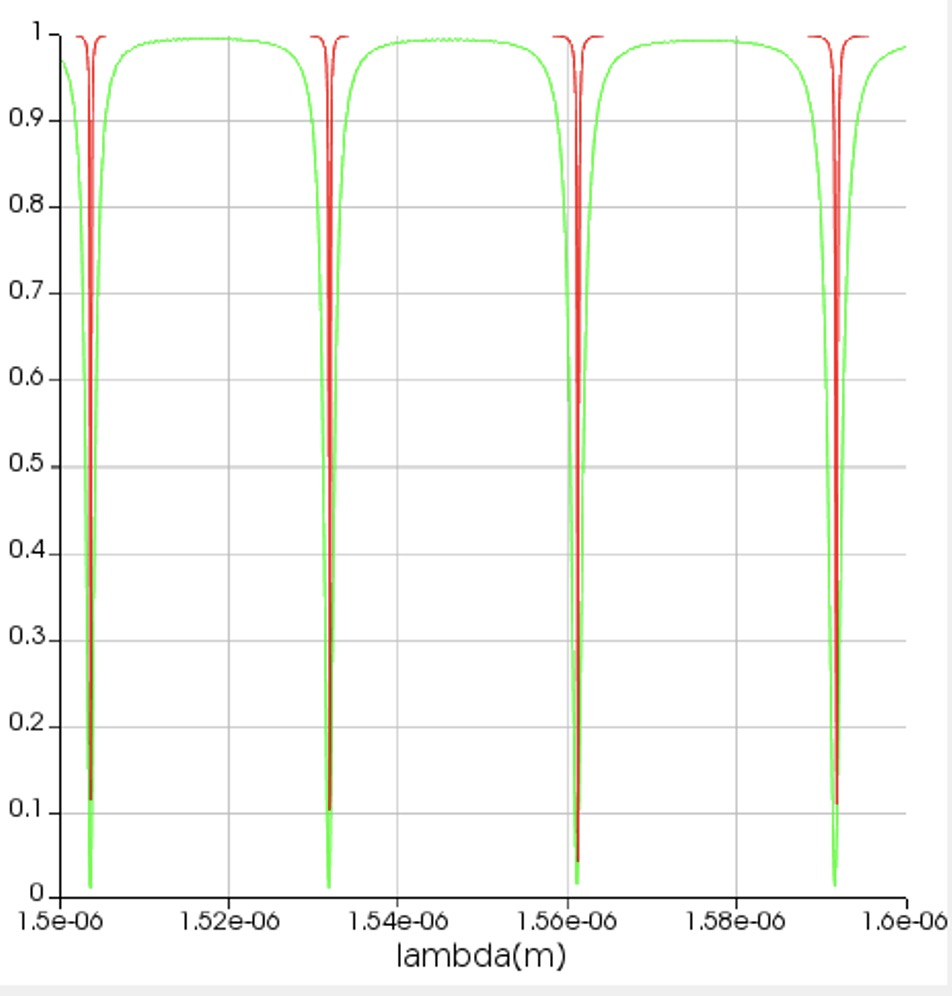
\includegraphics[width=1\textwidth]{img/fig3.3.png}
    \caption{The transimission when $\tau$ changes in $0.9, 0.7, 0.5, 0.3$
    along the row and $\tau_{\mathrm{middle}}$ changes in $0.9, 0.7, 0.5$ along
    the vertical columns}
    \label{fig3.2}
\end{figure}

%=================================================================================================
\pagebreak
%=================================================================================================
=======================================================================

\end{document}